% Using a4paper and 12pt font by default
\documentclass[12pt, a4paper]{article}

\usepackage[polish, british]{babel}

% Bibliography
\usepackage[backend=biber, giveninits=true, natbib=true, style=numeric, sorting=nty]{biblatex}
\addbibresource{references.bib}

\DeclareNameAlias{sortname}{family-given}
\DeclareNameAlias{default}{family-given}

% Use more than one optional parameter in a new commands
\usepackage{xargs}

% Colored text etc.
\usepackage[pdftex,dvipsnames]{xcolor}

% Quotation marks
\usepackage[utf8]{inputenc}

% Pictures and /includegraphics
\usepackage[final]{graphicx}
\usepackage{wrapfig}
\usepackage{float}

% Links in the table of contents + other stuff
\usepackage[hidelinks, linktoc=all]{hyperref}

% Support multi-page code listings
\usepackage[all]{hypcap}
\usepackage{subcaption}

% Times New Roman font
\usepackage[T1]{fontenc}
\usepackage{newtxmath,newtxtext}

% Margins
\usepackage[margin=2.5cm]{geometry}

% Interline
\usepackage{setspace}
\setstretch{1.5}

% Footnotes
\usepackage[bottom]{footmisc}

% Captions
\usepackage{caption}

% Code highlighting
\usepackage{minted}
\usemintedstyle{tango}

% New line after paragraph title
\newcommandx{\myparagraph}[1]{\paragraph{#1}\mbox{}}

% List stuff easily
\usepackage{multicol}
\usepackage[sharp]{easylist}

\let\OldEasylist\easylist
\let\OldEndEasylist\endeasylist
\renewenvironment{easylist}{%
    \OldEasylist%
    \ListProperties(Progressive*=3ex, Start1=1)%
}{%
    \OldEndEasylist%
}%

% Listing & picture counter
\usepackage{chngcntr}
\counterwithin{listing}{section}
\counterwithin{figure}{section}
\counterwithin{table}{section}

% Unbold the subsubsection and paragraph
\usepackage{titlesec}

\titleformat*{\subsubsection}{\normalfont\fontsize{13pt}{13pt}\selectfont}
\titleformat*{\paragraph}{\normalfont\itshape}

% Paragraph numbers
% \setcounter{secnumdepth}{4}


% Double abstract
% \newenvironment{abstractpage}
%   {\cleardoublepage\vspace*{\fill}\thispagestyle{empty}}
%   {\vfill\cleardoublepage}
% \renewenvironment{abstract}[1]
%   {\bigskip\selectlanguage{#1}%
%    \begin{center}\bfseries\abstractname\end{center}}
%   {\par\bigskip}

% Title page
\usepackage{pdfpages}

% Hyphenation rules, etc.
\usepackage{csquotes}

\begin{document}

% Title page
\includepdf[pages={1}]{title_page.pdf}

% Special page
\vspace*{\fill}
\begin{center}
The writing of the thesis has been requested.
\end{center}
\vspace{\fill}
\newpage

% Table of Contents
\tableofcontents
\newpage

% Abstract

\vspace*{\fill}
\begin{otherlanguage}{polish}
\begin{abstract}
    W dzisiejszych czasach znaczenie analizy dużej objętości danych staje się bardziej i bardziej oczywista. Coraz więcej firm decyduje się otworzyć dział analizy danych w celu poprawy własnej oferty; inne z analizy danach utworzyły ofertę dla innych firm. Praca inżynierska prezentuje wybrane metody analizy danych oferowane przez środowisko programowania Python, szeroko wykorzystanym w dziedzinie teorii informacji. Szczególną uwagę poświęcono na pokazaniu czytelnikowi przykładów, jak można wykorzystać Python dla analizy danych z publicznie dostępnych źródeł przez prezentacje kodu z różnych projektów, jak i przykładowych wyników, które mogą zostać uzyskane.
\end{abstract}
\end{otherlanguage}
\smallskip
\begin{abstract}
  The importance of analyzing large volumes of data is becoming more and more apparent in the modern era. An increasing number of companies decide to open a data analysis department in order to improve their offerings, and some of them even base their product around analyzing data for other people. This work presents some of the data analysis methods using the Python programming language environment, which is widely used in the domain of data science. It focuses on showing the reader examples of how one can use Python to analyze data from publicly available sources by presenting the source code of different projects as well as the results that it generates.
\end{abstract}
\vspace{\fill}
% \begin{abstractpage}
%   \begin{abstract}{polish}
%
%   \end{abstract}
%
%   \begin{abstract}{british}
%
%   \end{abstract}
%
% \end{abstractpage}




%===============================================================================
\newpage
\section{INTRODUCTION}
%===============================================================================

%-------------------------------------------------------------------------------
\subsection{Goals of the Research}
%-------------------------------------------------------------------------------
In the modern world, big data and machine learning are becoming more and more prominent as companies such as Facebook, Google and Amazon gather and analyze all sorts of data from their users. But which tools are they using to do it?

Right now, the two main languages in data science are Python \cite{popularlanguages} and R, while Java is the third by popularity and Matlab is also quite popular despite only being used in the academic environment.

This work's objective is to show how to use the Python 3 programming language in dealing with different kinds of data, and to help clarify any problems that might come up. It may be useful for long-term users of other languages that want to try Python out as well as users of Python 2, support for which will be stopped in 2020.
%-------------------------------------------------------------------------------
\subsection{Thesis Overview}
%-------------------------------------------------------------------------------
This work will be split into three parts, each working with a different dataset.

The first project is dealing with the time series data, using the last 17 years' worth of stock data from NYSE\footnote{New York Stock Exchange}.

The second project is dealing with the YouTube network, and is mostly showcasing different kinds of plots that you can make using the igraph and datashader packages. It also involves community detection.

The third project is dealing with the geographical data from the world bank\cite{world_bank_source}.

Lastly, the fourth part will contain conclusions.

%===============================================================================
\newpage
\section{TIME SERIES DATA ANALYSIS}
%===============================================================================
%-------------------------------------------------------------------------------
\subsection{Project Overview}
%-------------------------------------------------------------------------------

\subsubsection{Goals}

\begin{itemize}
	\item To show how to use python to obtain stock price data
	\item To show how to visualize the aforementioned data using both traditional single stock visualizations methods as well as some more unorthodox ones like a correlation heatmap
	\item To show how to predict future stock prices by using a LSTM neural network
\end{itemize}

\subsubsection{Description}

This project will focus on dealing with time series data, which will be represented by the stock price data. It will contain four sections.

In the first one, I will show how to use the pandas-datareader package to download stocks traded on the New York Stock Exchange (NYSE) from the Yahoo! finance website and merge them into one comma separated file.

In the second section, I will cover simple visualizations of singular stocks using the pandas\cite{mckinney2010data_pandas} and matplotlib\cite{hunter2007matplotlib} packages, which will include moving average and candlestick plots.

In the third section, I will cover visualization of a stock correlation matrix, which will, as opposed to the simple plots, include all of the stocks that were downloaded and not only one of them.

In the fourth and final section, I will demonstrate how to make a LSTM neural network for predicting the stock prices using the keras package and how to plot the predictions it generates, as well as cover how to use the pickle package to serialize python objects.


%-------------------------------------------------------------------------------
\newpage
\subsection{Data gathering (pandas-datareader)}
%-------------------------------------------------------------------------------

\subsubsection{Goals}

The goal of this section is to show how to use python to obtain stock price data, and transform it for further use.

\subsubsection{Downloading the data}

\begin{figure}[H]
    \centering
    \includegraphics[width=\textwidth]{src/stocks/etl/stocks_download_chart}
    \caption{Stocks download flowchart}
    \label{fig:stocks_download_chart}
\end{figure}

As you can see on the figure \ref{fig:stocks_download_chart}, the download process can only begins after you have specified the tickers, or short names of the companies that you want to download the data for.

There are a couple of methods to obtain a list of tickers that you want to analyze: you could go through the companies that interest you and look up the ticker for every one of them, you could use a package called BeautifulSoup to obtain the tickers by scraping a webpage, or, if you are dealing with all of the stocks traded on a particular market (like we are here with NYSE), the official webpage for that market usually provides such a list. In this case, I have downloaded a list of all tickers from NYSE from the official NASDAQ website \cite{nasdaq_companylist} and saved the ticker column from the provided file  manually.

It is possible to just go trough them one by one and call the download function for every ticker, but that approach may be detrimental due to the fact that sometimes Yahoo! Finance’s API  just outright refuses the pandas-datareader’s connection attempts, probably due to a large number of requests from one IP address.

Due to this inconsistency, we have to incorporate some fail-saves into the code, like checking whether the download was completed successfully and repeating it if something went wrong. The timeout between tries is also introduced here to avoid stressing the Yahoo! servers too much, and to avoid being flagged as a malicious user.

After a stock is processed this way, we save the data if we have successfully downloaded it, and go to the next stock in the list. While this approach doesn’t guarantee that 100\% of the stocks will get downloaded, it protects us from being stuck in an infinite loop due to Yahoo! Finance not having a data for a certain stock.

\myparagraph{Used packages}

Below you will find packages that will be used in this section of the project.

\bgroup
  \inputminted[linenos, breaklines=true, fontsize=\scriptsize, firstnumber=last]{python}{src/stocks/etl/0a_imports.py}
  \captionof{listing}{Imports}
  \label{listing:setl_0a_imports}
\egroup


\myparagraph{Tqdm}

Please pay attention to the use of the tqdm package in the listing \ref{listing:setl_1_download}. It is a very useful package that allows you to create progress bars that work in both console and jupyter notebooks, and help with determining how much time is left in a long process, or how many things we have already processed. To use it, you can just change \texttt{for i in iterable} to \texttt{for i in tqdm(iterable)}. And if you want to use it in while loops, you can create a tqdm object yourself and manually update it, as is is shown in the listing.

\bgroup
  \inputminted[linenos, breaklines=true, fontsize=\scriptsize]{python}{src/stocks/etl/1_download.py}
  \captionof{listing}{Downloading the stocks data}
  \label{listing:setl_1_download}
\egroup

\subsubsection{Data Transformation}

After downloading the stocks, we are left with a lot of files, where every file represents the data for a single stock. And this is a problem if we want to run some computations that involve every stock, since then we would need to loop through all the individual files in order to achieve that. That’s why in this subsection I’ll show how to merge all those files in one CSV file.

There are a couple of ways to accomplish this, but the one I find the most useful is to make numpy\cite{walt2011numpy} arrays out of the files, and then use the \texttt{np.concatenate} function to merge them. It is even possible to convert the resulting numpy array to a dataframe afterwards.

But there is one problem with this method. In order to  concatenate two numpy arrays, they must have the same number of rows (or columns, depending on which axis you are using to concatenate the arrays). And even though we have specified that we want data in a time period between 2000 and 2017, not every stock will actually have those dates in their CSV file. Since if a company had their IPO\footnote{Initial Public Offering - the first time that the company can be traded} after 2000, their file will start with the date that the stock could be traded.

In order to merge the files despite this, it is necessary to first go through every file list and make sure that they have the same number of rows inside, even if some of those rows are null. In order to do this, we can handpick one file to serve as an example, and then assign that file’s index to every other file. You can observe this process in listing \ref{listing:setl_2c_reindex}.

\bgroup
  \inputminted[linenos, breaklines=true, fontsize=\scriptsize, firstnumber=last]{python}{src/stocks/etl/2b_timearr.py}
  \captionof{listing}{Extracting a time array (index) from a file}
  \label{listing:setl_2b_timearr}
\egroup

You can see a usage of generators in the listing \ref{listing:setl_2a_listcsv}. A generator can usually be distinguished by the use of the \texttt{yield} keyword, and is essentially a function that is treated as an iterable. If a you have a function that generates large amounts of data, your program can benefit drastically from using generators, since everything is generated on the fly and you don't have to store the whole resulting list in memory.

\bgroup
  \inputminted[linenos, breaklines=true, fontsize=\scriptsize, firstnumber=last]{python}{src/stocks/etl/2a_listcsv.py}
  \captionof{listing}{Listing all csv files in a directory}
  \label{listing:setl_2a_listcsv}
\egroup

\bgroup
  \inputminted[linenos, breaklines=true, fontsize=\scriptsize, firstnumber=last]{python}{src/stocks/etl/2c_reindex.py}
  \captionof{listing}{Reindexing the files for future concatenation}
  \label{listing:setl_2c_reindex}
\egroup

One other problem that arises with merging the files is how to deal with columns being called the same way in every file. In this example, I have decided to solve it by appending the company name to every column, so we can still access data from a specific company in the future.

\bgroup
  \inputminted[linenos, breaklines=true, fontsize=\scriptsize, firstnumber=last]{python}{src/stocks/etl/2d_merge.py}
  \captionof{listing}{Merging the singular stock files}
  \label{listing:setl_2d_merge}
\egroup

A correlation matrix serves as a way to store relationships between stocks, and will be covered later in the section \ref{ssec:stock_corr}.

\bgroup
  \inputminted[linenos, breaklines=true, fontsize=\scriptsize, firstnumber=last]{python}{src/stocks/etl/2f_corr.py}
  \captionof{listing}{Creating a correlation matrix}
  \label{listing:setl_2f_corr}
\egroup


\subsubsection{Summary}

After defining all those functions, the only thing left now is to call them with correct arguments. As you can see from the listing \ref{listing:setl_3}, I use a datetime package from python’s standard library to specify the date ranges that I want to retrieve the data for, and in this case it’s from 2000 until 2017.

\bgroup
  \inputminted[linenos, breaklines=true, fontsize=\scriptsize, firstnumber=last]{python}{src/stocks/etl/3_executing.py}
  \captionof{listing}{Executing the functions}
  \label{listing:setl_3}
\egroup

To sum up, while the pandas-datareader module requires a lot of extra checking to ensure that the data was actually downloaded, it simplifies the process of web scraping tremendously, since you can just call a function that accesses certain provider’s API by itself. And despite it being limited by the number of providers you can access with it, I would say that the benefit of not having to parse the html or json yourself can play a significant role in programmers choosing this package over plain old web scraping.



%-------------------------------------------------------------------------------
\newpage
\subsection{Traditional stock visualizations (matplotlib)}
%-------------------------------------------------------------------------------
\subsubsection{Goals}
The goal of this section is to show how to use matplotlib to plot some of the more traditional single stock visualizations.


\subsubsection{Before plotting}
\myparagraph{Imports}

The packages that will be used in this section are listed in the listing \ref{listing:ssimp_0_imports} below.

\bgroup
  \inputminted[linenos, breaklines=true, fontsize=\scriptsize]{python}{src/stocks/simple/0_imports.py}
  \captionof{listing}{Imports}
  \label{listing:ssimp_0_imports}
\egroup

\myparagraph{Data loading}

We don't need to do any preparations in this section except for loading the data in memory. Please note the usage of \texttt{plt.style.use('seaborn')} in the listing \ref{listing:ssimp_1} - it changes the default simple looking style of matplotlib plots into a one that looks more modern.

\bgroup
  \inputminted[linenos, breaklines=true, fontsize=\scriptsize, firstnumber=last]{python}{src/stocks/simple/1_get_data.py}
  \captionof{listing}{Reading the data into the memory}
  \label{listing:ssimp_1}
\egroup

\subsubsection{Basic plot}

A basic plot of one stock can be plotted without having to resort to creating your own plot in matplotlib, since a pandas DataFrame has a built-in plot function. In this example, I created an empty matplotlib figure first, then plotted the stock data on top of it and displated the figure using the \texttt{plt.show()} function. You can also call \texttt{plt.savefig('filename.pdf')} instead, if you want to save your plot to a file, or just click the save icon in the interactive window that \texttt{plt.show()} generates.

\bgroup
  \inputminted[linenos, breaklines=true, fontsize=\scriptsize, firstnumber=last]{python}{src/stocks/simple/2_onestock.py}
  \captionof{listing}{Very basic plot of a stock}
  \label{listing:ssimp_2}
\egroup

\begin{multicols}{2}
{\centering
\includegraphics[width=\columnwidth]{src/stocks/simple/oneplot}\\
\captionof{figure}{Basic plot}
\label{fig:stock_oneplot}}
{\centering
\includegraphics[width=\columnwidth]{src/stocks/simple/oneplot_zoom}\\
\captionof{figure}{Basic plot - zoomed}
\label{fig:stock_oneplot_zoom}}
\end{multicols}

\subsubsection{Moving average plot}

In this subsection, I will show how to create a moving average plot. Moving average plots are used by analysts because they help to bring forward long-term trends and serve as a measure to smooth out outliers.

In pandas, you can create a special column that keeps track of the moving average of last \texttt{n} days by using the command \texttt{df['column'].rolling(window=n).mean()}. Then, you can use this newly generated column as another input for the \texttt{plot} function, and plot the moving average and the close price on the same figure. You can also do this process for different values of n and plot multiple moving averages to compare them - if a MA with a smaller \texttt{n} rises and crosses the MA with a larger \texttt{n}, it means that the raise in the stock price is substantial and it might be worth it to invest in such a stock.

I would also like to mention the \texttt{subplot2grid((y, x), (posy, posx))} function that you can see in the example - it breaks the figure down into an y by x grid, and allows you to pick a point that you would like to position a new axis object in. \texttt{rowspan} and \texttt{colspan} are used to determine how many rows or columns respectively this part of the plot should take.

\bgroup
  \inputminted[linenos, breaklines=true, fontsize=\scriptsize, firstnumber=last]{python}{src/stocks/simple/3_moving_avg.py}
  \captionof{listing}{Moving average plot}
  \label{listing:ssimp_3}
\egroup

\begin{figure}[H]
    \centering
    \includegraphics[width=\textwidth]{src/stocks/simple/movingavg}
    \caption{Moving average plot}
    \label{fig:stock_movingavg}
\end{figure}

\begin{figure}[H]
    \centering
    \includegraphics[width=\textwidth]{src/stocks/simple/movingavg_zoom}
    \caption{Moving average plot - zoomed}
    \label{fig:stock_movingavg_zoom}
\end{figure}

\subsubsection{Candlestick plot}

A candlestick plot is a way to visualize aggregated stock data that has originated in Japan and was popularized in the west by Steve Nison \cite{candlestick}. It employs a structure that is similar to box plots to show the stock’s opening, close, high and low prices for a specific time period - usually a day or a week. Usually, a entry for one day (or week, month, etc.) consists of the following: (1) a box, showing opening and close prices and (2) lines, or “shadows”, that show the high and low prices (you can see those on figure \ref{fig:stock_candlestick_zoom}). This, in combination with changing the color of the box to show whether the stock has gone up or down in price to create this plotting technique. Candlestick plotting is also often combined with a volume plot that shows how much trading was done in that time period (on the bottom in the example).

\begin{figure}[H]
    \centering
    \includegraphics[width=\textwidth]{src/stocks/simple/candlestick_zoom}
    \caption{Candlestick plot - zoomed}
    \label{fig:stock_candlestick_zoom}
\end{figure}

The pandas package has some support for the candlestick plots, which, as you can see in the listing \ref{listing:ssimp_4_candle}, can be very useful when trying to create such plots by yourself.  You can use functions like \texttt{df[column].resample('time\_period')} to resample your data and then pair it with \texttt{df.ohlc()} to extract the open/high/low/close values from that aggregation. This, paired with \texttt{candlestick\_ohlc} function from \texttt{matplotlib.finance} module allows you to create candlestick plots rather quickly.

\bgroup
  \inputminted[linenos, breaklines=true, fontsize=\scriptsize, firstnumber=last]{python}{src/stocks/simple/4_candlestick.py}
  \captionof{listing}{Candlestick chart}
  \label{listing:ssimp_4_candle}
\egroup

As you can see in the figures \ref{fig:stock_candlestick_zoom} above and \ref{fig:stock_candlestick} below, the resulting plot is interactive and allows for the user to zoom in and only view the time period that they are interested in.

\begin{figure}[H]
    \centering
    \includegraphics[width=\textwidth]{src/stocks/simple/candlestick}
    \caption{Candlestick plot}
    \label{fig:stock_candlestick}
\end{figure}


%-------------------------------------------------------------------------------
\newpage
\subsection{Stock correlation matrix visualization (matplotlib)} \label{ssec:stock_corr}
%-------------------------------------------------------------------------------

\subsubsection{Goals and section overview}

\myparagraph{Goal}

The goal of this section is to show, how you can visualize a stock correlation matrix, as well as to discuss the necessity of such visualization.

\myparagraph{Correlation matrix}

A correlation between two stock prices shows, whether a rise in price of one stock correlates with a rise or fall in price of another stock, or whether two stocks are completely independent.

A logical, albeit a bit inefficient, way to store correlation between a certain number of stocks is to create a so-called correlation matrix, whose structure you can see in table \ref{table:corr}.

Some research\cite{kwapien2006bulk} suggests that correlation matrix may contain useful information about the stock market, which makes it into a metric that can be used by stock investors that would like to diversify their investment portfolio as much as possible, thus ensuring that if one of the stocks they have invested in drops in price, the other ones remain stable.

\begin{table}[h!]
\centering
\caption{Correlation matrix structure}
\begin{tabular}{ | c | c | c | c | }
  \hline
  \ & Stock1 & Stock2 & Stock3 \\
  \hline
  Stock1 & 1 & corr(Stock1, Stock2) & corr(Stock1, Stock3) \\
  \hline
  Stock2 & corr(Stock2, Stock1) & 1 & corr(Stock2, Stock3) \\
  \hline
  Stock3 & corr(Stock3, Stock1) & corr(Stock3, Stock2) & 1 \\
  \hline
\end{tabular}
\label{table:corr}
\end{table}

Once we have this matrix, a question arises - how can we visualize it? In this example visualization, I'll use a heat map chart, because of how the correlation numbers can be treated as colors.

\bgroup
  \inputminted[linenos, breaklines=true, fontsize=\scriptsize]{python}{src/stocks/corr/0_imports.py}
  \captionof{listing}{Imports}
  \label{listing:scorr_0_imports}
\egroup

\bgroup
  \inputminted[linenos, breaklines=true, fontsize=\scriptsize, firstnumber=last]{python}{src/stocks/corr/1_get_data.py}
  \captionof{listing}{Reading the data into the memory}
  \label{listing:scorr_1}
\egroup

\subsubsection{Naive plot}

In this plot, I have used the \texttt{pcolormesh} function in order to create a heat map of the values from the df\_corr dataframe. Data didn’t require any extra preprocessing, since the correlations are already in a range \texttt{[-1:1]}, and that means that the colors will render properly.

Unfortunately, if you try to plot a heat map this large, some problems starts to occur with matplotlib. In this case, if just thought that the last cell to the right was a stock with a name starting with “A”, even though it should be something from the other part of the alphabet, like “Z”. And even if you try to zoom into the plot, those labels don’t update and continue to be wrong. I will cover how to deal with this problem by inheriting from a formatter class in the section \ref{sssec:correct_corr_plot}.

\bgroup
  \inputminted[linenos, breaklines=true, fontsize=\scriptsize, firstnumber=last]{python}{src/stocks/corr/2_problem_labels.py}
  \captionof{listing}{Correlation matrix - labels are broken}
  \label{listing:scorr_2}
\egroup

\begin{figure}[H]
    \centering
    \includegraphics[width=\textwidth]{src/stocks/corr/corr}
    \caption{Correlation plot (incorrect labels)}
    \label{fig:stock_corr}
\end{figure}

\subsubsection{Correct plot}\label{sssec:correct_corr_plot}

The default matplotlib tick formatter can’t dynamically update values. This means, that if I would want to set the ticks myself, I would have to display all of them on the screen at the same time, which just leads to all the labels overlapping with each other. But we can inherit from the matplotlib’s tick formatter class in order to solve this issue. As you can see in the listing \ref{listing:scorr_3}, you only have to override two functions from the parent class in order to achieve dynamic update of the labels, even if it does make the plot somewhat stutter when you use the interactive zoom feature.

I have also used the MaxNLocator, which is similar to the default matplotlib’s behavior - it will choose to use between min\_n\_ticks and nbins + 1 locations, and position them in “nice locations”, according to matplotlib’s documentation. Both of those variables are keyword arguments to its \_\_init\_\_ function, and can easily be changed.

I would also like to point out, that while it can’t be seen in the figures below, if you mouseover a cell in the heat map while being in an interactive mode, the program displays you the stocks that the chosen cell represents.

\bgroup
  \inputminted[linenos, breaklines=true, fontsize=\scriptsize, firstnumber=last]{python}{src/stocks/corr/3_fix.py}
  \captionof{listing}{Fixing the labelling}
  \label{listing:scorr_3}
\egroup

\begin{figure}[H]
    \centering
    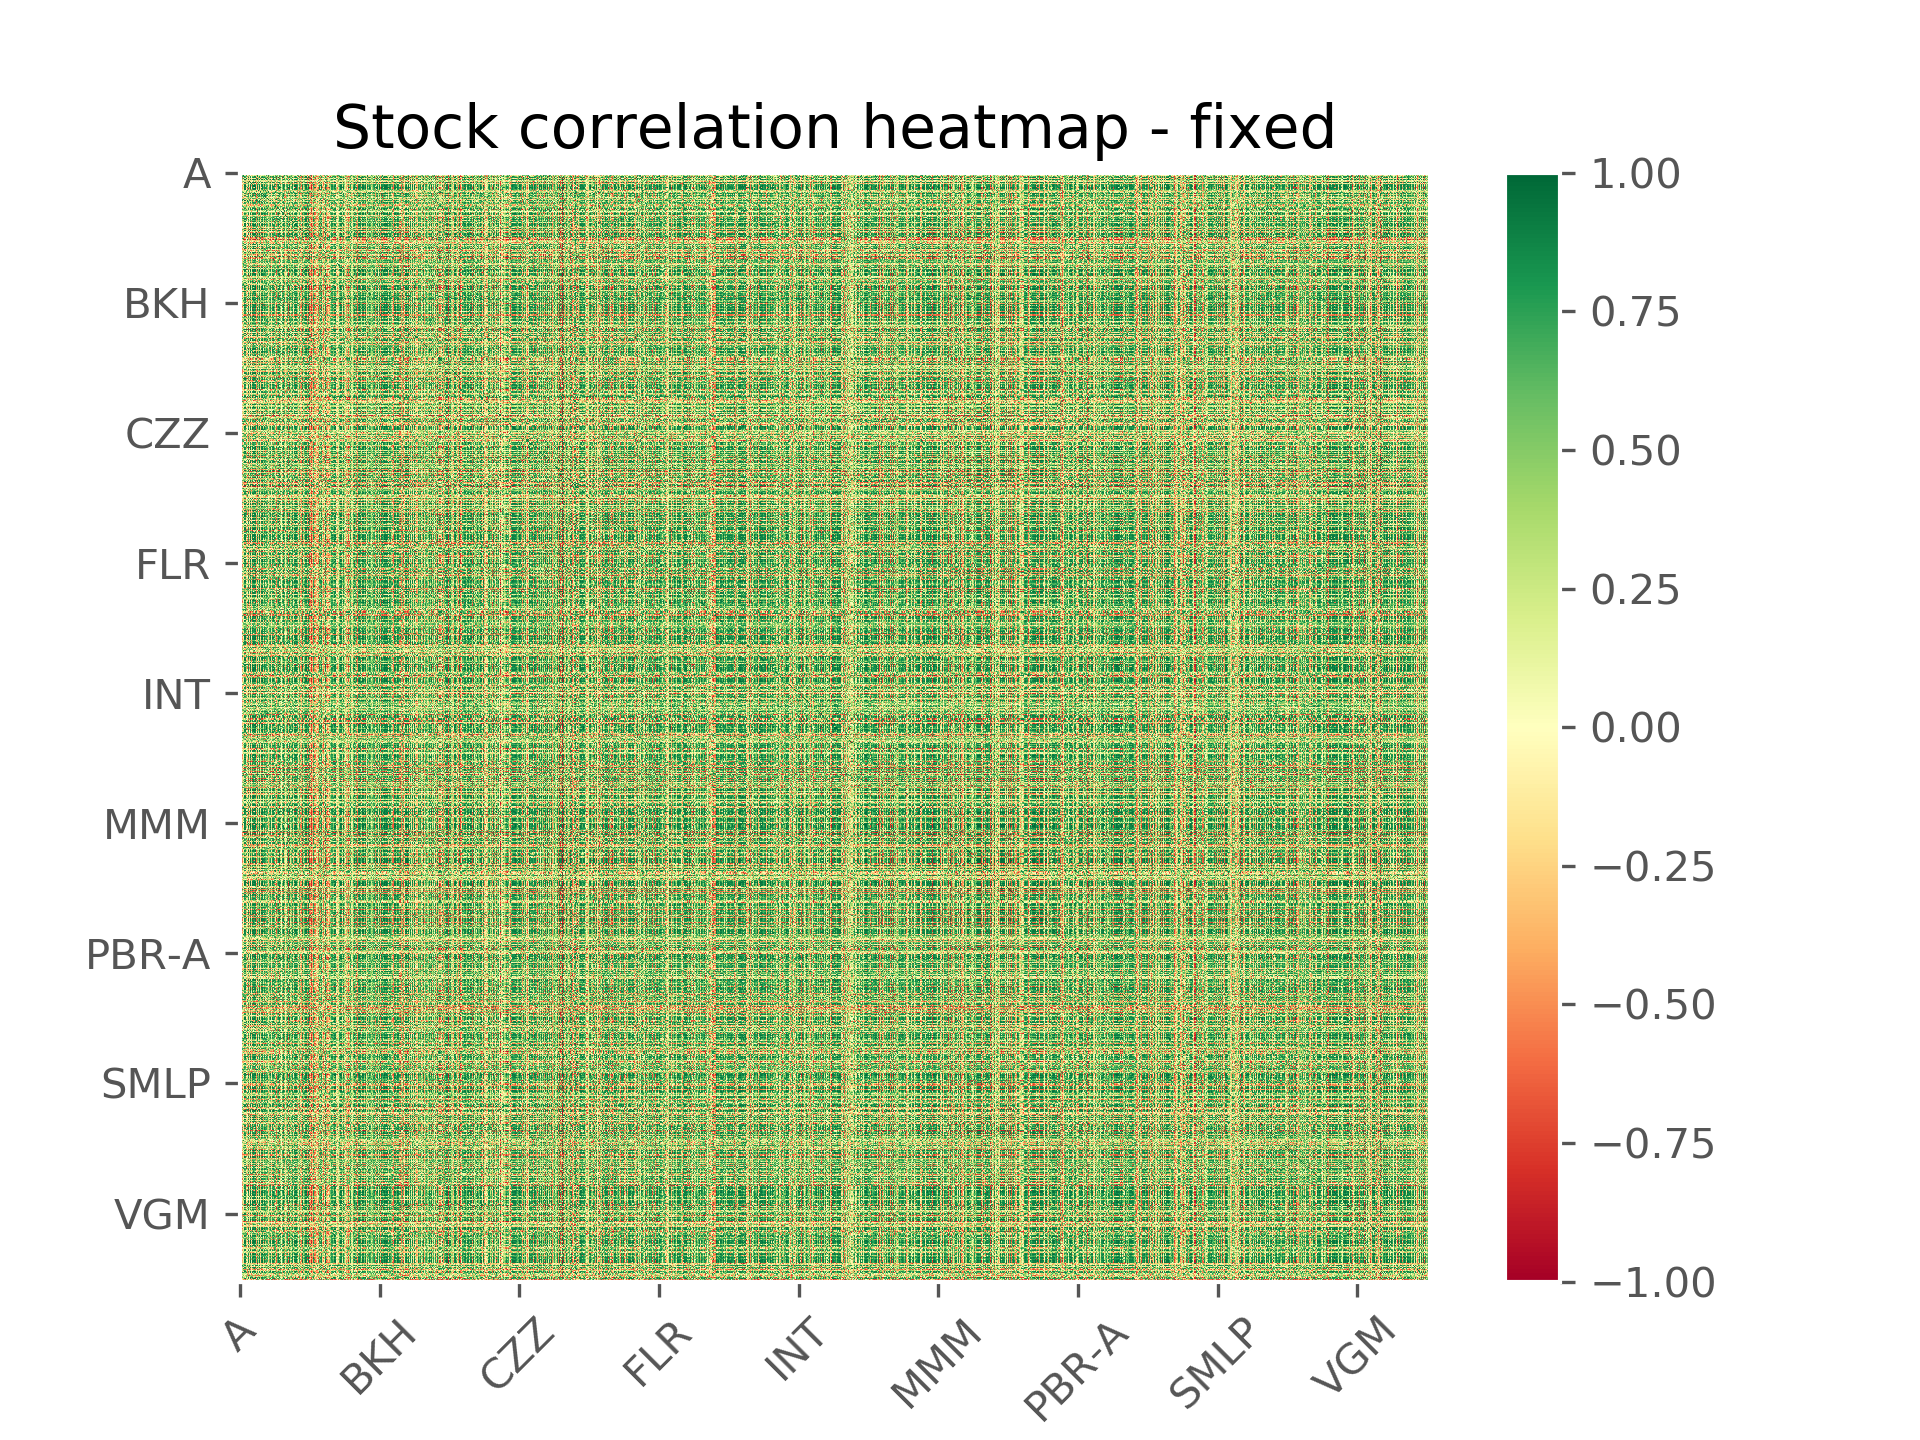
\includegraphics[width=0.9\textwidth]{src/stocks/corr/corr_fix}
    \caption{Correlation plot (fixed)}
    \label{fig:stock_corr_fix}
\end{figure}

\begin{figure}[H]
    \centering
    \includegraphics[width=0.9\textwidth]{src/stocks/corr/corr_fix_zoom}
    \caption{Correlation plot (fixed) - zoomed}
    \label{fig:stock_corr_fix_zoom}
\end{figure}

\subsubsection{Summary and necessity of plotting the matrix}

In retrospective, I would say that there are problems with this plot simply because it’s too cluttered and hard to understand. You have to zoom in whenever you want to actually see the correlation between some stocks and not just some vague green or red lines. However, once zoomed in it becomes quite easy to check the correlation between two plots. I think that it could be improved by either focusing more on the neutrally correlated stocks, and making the highly positive and highly negative areas transparent, or by making the number of stocks that we have to show smaller. Since the current version displays all stocks from the market and is very hard to read due to the number of rows and columns being too high, I think that a version with 5, 10 or maybe even 20 stocks could be better since then you would actually see all of the date from a picture without having to zoom.

%-------------------------------------------------------------------------------
\newpage
\subsection{Predictive analysis with a LSTM neural network (keras)}
%-------------------------------------------------------------------------------
\subsubsection{Goals and project overview}

The goal of this section is to show how to predict future stock prices using a long short term memory neural networks.

\myparagraph{Project description}

A long short term memory neural network is a type of a recursive neural network, that was invented in 1997 by Hochreiter and Schmidhuber\cite{hochreiter1997long}. It replaces the standard neuron from a NN with a memory cell that not only learns how to predict something, but also how to forget something in order to be able to indentify long-term dependancies.

In this project, I will feed the neural network with the data for an entire NYSE stock market using the keras\cite{chollet2015keras} with tensorflow\cite{abadi2016tensorflow} backend, and try to predict the price of one stock based on that.

\myparagraph{Used packages}

\bgroup
  \inputminted[linenos, breaklines=true, fontsize=\scriptsize]{python}{src/stocks/lstm/0_imports.py}
  \captionof{listing}{Imports}
  \label{listing:slstm_0_imports}
\egroup

\subsubsection{Data preparation}

Loading the data in the memory is the same as in the plotting section, but now we will need to preprocess it into a format that is acceptable by keras.

\bgroup
  \inputminted[linenos, breaklines=true, fontsize=\scriptsize, firstnumber=last]{python}{src/stocks/lstm/1_data.py}
  \captionof{listing}{Loading data into the memory}
  \label{listing:slstm_1_data}
\egroup


\myparagraph{Preprocessing}

A LSTM NN requires us to feed it input in sequential blocks of data and not just block by block like a regular NN - this utilizes the memory function of the lstm neurons, and allows for these types of networks to predict next entry in a dataset (movie frames, stock prices, human speech, etc.). For the purpose of this example, I have chosen for the block size to be 30 days. It means, that we have to split out current dataset into 30-day continuous chunks. You can see me do it in the lines 59-67 of the listing \ref{listing:slstm_2a_preprocessing}. I start with an empty arrays X and y, and then add slices of 30 days to them until I can no longer add any.

You can also see how it is possible to scale features to a range between 0 and 1 (which improve your neural network's results \cite{muller2016introduction} \cite{grus2015data}) by using scikit-learn's\cite{pedregosa2011scikit} built in MinMaxScaler as well as how to execute a Principal Component Analysis\cite{wold1987principal} with another scikit-learn object. PCA reduces the number of features in your dataset, and while it may be detrimental to the results, a smaller number of features makes your neural network train a lot faster.

\bgroup
  \inputminted[linenos, breaklines=true, fontsize=\scriptsize, firstnumber=last]{python}{src/stocks/lstm/2a_preprocessing.py}
  \captionof{listing}{Declaring the data preprocessing functions}
  \label{listing:slstm_2a_preprocessing}
\egroup

The split\_x\_y function is mostly a wrapper for the convert\_series function that converts the input dataframe into those window-sized chunks and splits the dataset into a train and a test set.

Please note the usage of the pickle package in the listing \ref{listing:slstm_2b_preprocessing_exec} - it can be very useful, since if you save your objects to the drive by pickling them you don't have to generate them again.

\bgroup
  \inputminted[linenos, breaklines=true, fontsize=\scriptsize, firstnumber=last]{python}{src/stocks/lstm/2b_preprocessing_exec.py}
  \captionof{listing}{Executing the data preprocessing functions}
  \label{listing:slstm_2b_preprocessing_exec}
\egroup

\subsubsection{Network creation}

Netork creation is rather simple using keras - you just have to initialize an instance of the \texttt{Sequential} class to serve as your model's base, and then you can start adding layers to it using the \texttt{add} function. While it's rather obvious that \texttt{LSTM} means Long Short Term Memory layer, a dense layer is a layer filled with regular neurons, and a dropout keyword argument shows how many neurons will be randomly reset on each run. While it may sound counterintuitive, it sometimes is beneficial and helps to avoid overfitting. The loss chosen in this example is a mean squared error loss, or ``mse'', if we use keras' terms. The optimizer chosen for this example is Adam, which has been shown to converge faster than other similar algorithms in the study that introduced it\cite{kingma2014adam}.

\bgroup
  \inputminted[linenos, breaklines=true, fontsize=\scriptsize, firstnumber=last]{python}{src/stocks/lstm/3a_onelayer.py}
  \captionof{listing}{Creating a neural network with one layer}
  \label{listing:slstm_3a_onelayer}
\egroup

\bgroup
  \inputminted[linenos, breaklines=true, fontsize=\scriptsize, firstnumber=last]{python}{src/stocks/lstm/3b_twolayer.py}
  \captionof{listing}{Creating a neural network with two layers}
  \label{listing:slstm_3b_twolayer}
\egroup

\subsubsection{Network training}

The \texttt{model.fit()} function in keras is used to train the network. It takes parameters like batch\_size, that indicates how many entries we want to process at once, epoch\_size, that shows how many times we want to go through the input dataset as well as validation\_split that shows what fraction of the train data should be left for validation.

But I would like to focus your attention on the callbacks parameter, since it is a very interesting feauture of keras that allows you to specify ``monitors"", that will watch the training and do something if their condition is satisfied. For example, you can look at the listing \ref{listing:slstm_4a_fit} and see how I defined an early stopping monitor that monitors \texttt{val\_loss} with the patience of 5 on line 168. It means, that if our val\_loss doesn't improve for 5 epochs in a row (which shows that adam has found a local minimum), it will stop the training, thus saving us a lot of time. That said, it won't be beneficial every time, since sometimes the found minimum isn't ideal and the algorithm can ``climb out"" of it.

\bgroup
  \inputminted[linenos, breaklines=true, fontsize=\scriptsize, firstnumber=last]{python}{src/stocks/lstm/4b_plot.py}
  \captionof{listing}{Plotting the results}
  \label{listing:slstm_4b_plot}
\egroup

\bgroup
  \inputminted[linenos, breaklines=true, fontsize=\scriptsize, firstnumber=last]{python}{src/stocks/lstm/4a_fit.py}
  \captionof{listing}{Training the network}
  \label{listing:slstm_4a_fit}
\egroup

\subsubsection{Results overview}

\begin{multicols}{2}
{\centering
\includegraphics[width=\columnwidth]{src/stocks/lstm/one_layer_pred}\\
\captionof{figure}{One layer network prediction}
\label{fig:lstm_pred_one}}
{\centering
\includegraphics[width=\columnwidth]{src/stocks/lstm/two_layer_pred}\\
\captionof{figure}{Two layer network prediction}
\label{fig:lstm_pred_two}}
\end{multicols}

\begin{table}[h!]
\centering
\caption{LSTM networks losses}
\begin{tabular}{ | c | c |}
  \hline
  One layer & Two layer \\
  \hline
  0.00934559645561 & 0.00476981351654 \\
  \hline
\end{tabular}
\label{table:lstm}
\end{table}

Looking at the results, it is clear that the a network with two layers has proven to be more accurate than a network with one layers. It is probably due to the large amounts of data that we tried to give to the networks - having two LSTM layers has helped in detecting more intricate dependencies. Of course, the obtained results could have been improved by testing more nodes/layers combinations as well as using different preprocessing techniques. I would also recommend using PCA in the data preprocessing step to reduce the number of input dimensions if your computer can not handle this amount of columns.

Also, please note how to load the model once you have it saved in the listing \ref{listing:slstm_5_results}. Once you have saved a keras model to an HDF5 file using \texttt{model.save()}, you can load it back in and be ready to make predictions by using \texttt{load\_model()}.

\bgroup
  \inputminted[linenos, breaklines=true, fontsize=\scriptsize, firstnumber=last]{python}{src/stocks/lstm/5_results.py}
  \captionof{listing}{Obtaining the final plots and losses}
  \label{listing:slstm_5_results}
\egroup

\begin{multicols}{2}
{\centering
\includegraphics[width=\columnwidth]{src/stocks/lstm/one_layer}\\
\captionof{figure}{One layer network structure}
\label{fig:lstm_structure_one}}
{\centering
\includegraphics[width=\columnwidth]{src/stocks/lstm/two_layer}\\
\captionof{figure}{Two layer network structure}
\label{fig:lstm_structure_two}}
\end{multicols}





%===============================================================================
\newpage
\section{GRAPH DATA ANALYSIS}
%===============================================================================
%-------------------------------------------------------------------------------
\subsection{Project Overview}
%-------------------------------------------------------------------------------
\subsubsection{Goals}
The goals of this project are the following:

\begin{itemize}
\item To show how to run community detection algorithms in igraph
\item To show how to plot the communities using two different methods - datashader  (larger data) and igraph/cairo (smaller data)
\item To show how to make the communities visually separable and how to incorporate node weights in the plot
\end{itemize}

\subsubsection{Description}
This project will focus on processing graph data using the igraph package for Python that is built on top of the C library with the same name \cite{csardi2006igraph} and visualizing it using datashader \cite{ref_datashader} and plotting functions that are built into igraph. The data source for this project is a graph of the YouTube social network from 2007, that was downloaded from The Koblenz Network Collection \cite{youtube_source}.

In the first section I will focus on reading the obtained files and importing it in the Python environment by creating an \texttt{igraph.Graph()} object. I will also show how to detect communities in an igraph by using such algorithms as louvain\cite{blondel2011louvain} and infomap\cite{rosvall2008maps_infomap}.

In the second section, I will cover visualization of the whole graph as well as a large subsection of the graph using datashader.

In the third section, I will cover visualization of a smaller subsection of the graph using the plotting methods that are built into igraph.

\subsubsection{Packages used}

Below you can find the imports that will be used in the entire project

\bgroup
  \inputminted[linenos, breaklines=true, fontsize=\scriptsize]{python}{src/youtube/0_imports.py}
  \captionof{listing}{Imports}
  \label{listing:youtube_0_imports}
\egroup

%-------------------------------------------------------------------------------
\newpage
\subsection{Preprocessing, igraph creation and community detection}
%-------------------------------------------------------------------------------
\myparagraph{Goal}

The goal of this section is to show how to load a graph from an edge list file, as well as to show how to detect communities in a graph.

\myparagraph{Pandas dataframe}

The source file for this project is a file called ``out"" with no extentions. But if you read it using a text editor, you will see that it is just a regular delimited file that uses spaces as a separator and is, essentially, an edge matrix.

Please note how to skip rows (there were comments in the file) and define a custom separator when reading a DataFrame using keyword arguments.

\bgroup
  \inputminted[linenos, breaklines=true, fontsize=\scriptsize]{python}{src/youtube/igraph_creation/1_pandas.py}
  \captionof{listing}{Using pandas to load the initial data source}
  \label{listing:youtube_1_pandas}
\egroup

\myparagraph{igraph creation}

igraph utilizes its own system of numbering vertices and edges - they must be sequential and start from zero. But the source file starts numbering vertices from one, and has breaks in the numbering, so, for example, vertice 17 can be followed by vertice 25 instead of vertice 18. This means, that we have to rename the vertices and edges ourselves, while maintaining the proper edge information.

In the listing \ref{listing:youtube_2_igraph}, I start with creating an empty \texttt{igraph.Graph} object. Then I use a \texttt{np.ravel()} to flatten out the edge matrix, and then select unique vertice names from it using \texttt{pd.unique()} function. After obtaining this list of vertice names, I can use its length to create a continuous sequence of numbers starting with zero using \texttt{np.arange(start, end)} that will replace the vertice names. I proceed by adding that sequence to a graph by using the \texttt{add\_vertices} function.

I have to map vertice numbers from the edge matrix to the new continuous list to be able to import it into igraph. First step in doing that is to use builtin \texttt{dict} and \texttt{zip} functions to create a dictionary where a vertice real name is the key and the sequential number is the value. As you can see from the listing, \texttt{zip(it1, it2)} function is very useful - it takes two iterators as an input and then outputs a iterator that returns tuples \texttt{(it1[i], it2[i])} when called an ith time. In here, I have used the \texttt{dict} function to instantly convert that tuple iterator to a disctionary. Then, I use the \texttt{np.vectorize(function)} function, that converts a function from a one that takes one element of an array as an argument to a one that takes the entire array as an argument, and executes the old function on every element of that array. I have also used a lambda expression here. A lambda expression in Python is a short-hand way to define a function that doesn't require using \texttt{def} and proper spacing. But, since it is only a short-hand after all, you can't execute more than one command using the lambda expression. Thankfully, this time we only have to look up the old vertice name in the dictionary and get the new name out of it, and a dictionary lookup only takes one command. After executing the vectorized function on the edge matrix, the result are ready to be imported into igraph, which I do by using the \texttt{add\_edges()} function.

\bgroup
  \inputminted[linenos, breaklines=true, fontsize=\scriptsize, firstnumber=last]{python}{src/youtube/igraph_creation/2_igraph.py}
  \captionof{listing}{Creating an igraph}
  \label{listing:youtube_2_igraph}
\egroup

\myparagraph{Community detection}

You can see the community detection code in the listing \ref{listing:youtube_3_communities} below. It uses the louvain algorithm to partition the initial graph, and then switches to infomap to partition the smaller one. This is done this way, because the louvain algorithm was specifically developed and optimized for large graphs, while infomap requires us to perform some computationally expensive operations like walking the graph tree to find the communities.

\bgroup
  \inputminted[linenos, breaklines=true, fontsize=\scriptsize, firstnumber=last]{python}{src/youtube/igraph_creation/3_communities.py}
  \captionof{listing}{Detecting communities}
  \label{listing:youtube_3_communities}
\egroup


%-------------------------------------------------------------------------------
\newpage
\subsection{Plotting large graphs (datashader)}
%-------------------------------------------------------------------------------
\subsubsection{Goals}

\begin{itemize}
  \item To show how you can plot regular large graphs with datashader
  \item To show how you can plot large graphs while distinguishing communities in them
\end{itemize}

\subsubsection{Simple plot}

\myparagraph{Datashader introduction}

Datashader is a package that allows the user to visualize large amounts of data. It uses a lot of different aggregation techniques in order to generate plots that, while showing a lot of data, are possible to process and show.

\myparagraph{Description}

In this subsection, I have decided to try and plot the whole graph of the YouTube friends netwrok using datashader. I started with defining the following plot functions: plots\_edges, plot\_vertices and plot\_full that you can see in the listing \ref{listing:youtube_plot_functions}. All of them start out by creating a \texttt{ds.Canvas} object, that will be used as a matplotlib figure by datashader - all plots, points, lines will be plotted on that canvas.

As for what we will put on that canvas, Datashader works as follows: there are two types of graph functions you can call - a bundling function or a layout function. A bundling function is responsible for the edge placement, and the layout - for vertices. The bundling function is called that way, because datashader allows to aggregate edges into bundles, and we will cover that in the next subsection.

For the edge plot, I expect to receive that output of the bundling function that I will then just have to pass to the \texttt{canvas.line} function in order to plot the edges. And \texttt{ds\_tf.shade} is used as a compile function - once you shade your points, they are converted to an RGBA image.


For vertices it's the opposite - I expect to receive the output of the layout function that I can later pass to a \texttt{canvas.points} function.
The spread function in here helps to make vertices more visible by extending every pixel occupied by a vertice by a predefined value.

\bgroup
  \inputminted[linenos, breaklines=true, fontsize=\scriptsize]{python}{src/youtube/plot_functions.py}
  \captionof{listing}{Datashader plotting functions}
  \label{listing:youtube_plot_functions}
\egroup

In the full graph example I am using the random layout and directly connected edges bundling (in another words, no bundling at all) because when I have tried to run the bundling and a more complicated layout calculations on my data science server, it ran for three days and then just crashed. I assume that this graph was a tad too big for datashader to process.

\bgroup
  \inputminted[linenos, breaklines=true, fontsize=\scriptsize, firstnumber=last]{python}{src/youtube/datashader/simple/1a_prep.py}
  \captionof{listing}{Creating datashader layouts}
  \label{listing:youtube_lgr_1a}
\egroup

To plot these images in this case I've used a simple \texttt{ds\_tf.Image function}, that just displays an image. I will cover how to save them to a file in a next subsection.

\bgroup
  \inputminted[linenos, breaklines=true, fontsize=\scriptsize, firstnumber=last]{python}{src/youtube/datashader/simple/1b_plot.py}
  \captionof{listing}{Plotting the whole plot using datashader}
  \label{listing:youtube_lgr_1b}
\egroup

\myparagraph{Results}

\begin{multicols}{2}
{\centering
\includegraphics[width=\columnwidth]{src/youtube/datashader/simple/fullgraph_edges}\\
\captionof{figure}{Edge plot of the full graph}
\label{fig:ds_fullgraph_edges}}
{\centering
\includegraphics[width=\columnwidth]{src/youtube/datashader/simple/fullgraph_full}\\
\captionof{figure}{Full plot of the full graph}
\label{fig:ds_fullgraph_full}}
\end{multicols}

As you can see, no indormation can be obtained from the above figures. And while datashader is certainly capable of plotting a huge amounts of data points, sometimes using that capability is a bad idea and only leads to dissappointing results.

%- - - - - - - - - - - - - - - - - - - - - - - - - - - - - - - - - - - - - - - -
\subsubsection{Regular plot}
%- - - - - - - - - - - - - - - - - - - - - - - - - - - - - - - - - - - - - - - -

\myparagraph{Description}

In this subsection, I will show you how to plot a quite large subgraph (26000 vertices) of the YouTube graph using datashader. I am using the communities obtained by the louvain algorithm as vertices. I will also compare different layout and bundling combinations.

\myparagraph{Creating a plot list}

While the last subsection's results were quite dissappointing, the plotting functions used there are correct. Since in this subsection I will be comparing a lot of different layouts and bundlings, I have decided to create a list of these plots, and then just save them using a for loop. As you can see, I started with creating a one of every layout and then created a one of every bundling for those layouts. Then, I have created a list that includes every layout/bundling combination by just calling the plot functions from inside of the list declaration.

\bgroup
  \inputminted[linenos, breaklines=true, fontsize=\scriptsize]{python}{src/youtube/datashader/simple/2a_layouts.py}
  \captionof{listing}{Creating layouts}
  \label{listing:youtube_lgr_2a}
\egroup

\bgroup
  \inputminted[linenos, breaklines=true, fontsize=\scriptsize]{python}{src/youtube/datashader/simple/2b_showcase.py}
  \captionof{listing}{Creating a list with layout combinations}
  \label{listing:youtube_lgr_2b}
\egroup

\myparagraph{Saving the plot}

In order to save the plots, I have to iterate through the previously created list of layouts and us the \texttt{export\_image} function from datashaders.utils package to save the plots. Please not, how to use it, since it is much more convenient to save images using a specialized function than by saving an image from your jupyter notebook or just a regular python output. I have also used tqdm to show the progress of saving the images.

\bgroup
  \inputminted[linenos, breaklines=true, fontsize=\scriptsize, firstnumber=last]{python}{src/youtube/datashader/simple/2c_saving.py}
  \captionof{listing}{Saving the plots}
  \label{listing:youtube_lgr_2c}
\egroup

\myparagraph{Results}

\begin{figure}[H]
    \centering
    \begin{subfigure}[b]{\textwidth}
        \centering
        \includegraphics[width=0.33\textwidth]{src/youtube/datashader/simple/datashader/1_1}%
        \hfill
        \includegraphics[width=0.33\columnwidth]{src/youtube/datashader/simple/datashader/1_2}%
        \hfill
        \includegraphics[width=0.33\columnwidth]{src/youtube/datashader/simple/datashader/1_3}
    \end{subfigure}
    \caption{Circular layout - Bundled}
    \label{fig:ds_show_1}
\end{figure}

\begin{figure}[H]
    \centering
    \begin{subfigure}[b]{\textwidth}
        \centering
        \includegraphics[width=0.33\textwidth]{src/youtube/datashader/simple/datashader/2_1}%
        \hfill
        \includegraphics[width=0.33\columnwidth]{src/youtube/datashader/simple/datashader/2_2}%
        \hfill
        \includegraphics[width=0.33\columnwidth]{src/youtube/datashader/simple/datashader/2_3}
    \end{subfigure}
    \caption{Circular layout - Directly connected}
    \label{fig:ds_show_2}
\end{figure}

I would say that the circular layout overall is a quite bad way to represent large graphs, since you can't really see the connections between nodes once they are in a circle. While it may work with very small graphs, in here they are just pictures of a filled circle.

\begin{figure}[H]
    \centering
    \begin{subfigure}[b]{\textwidth}
        \centering
        \includegraphics[width=0.33\textwidth]{src/youtube/datashader/simple/datashader/5_1}%
        \hfill
        \includegraphics[width=0.33\columnwidth]{src/youtube/datashader/simple/datashader/5_2}%
        \hfill
        \includegraphics[width=0.33\columnwidth]{src/youtube/datashader/simple/datashader/5_3}
    \end{subfigure}
    \caption{Random layout - Bundled}
    \label{fig:ds_show_5}
\end{figure}


\begin{figure}[H]
    \centering
    \begin{subfigure}[b]{\textwidth}
        \centering
        \includegraphics[width=0.33\textwidth]{src/youtube/datashader/simple/datashader/6_1}%
        \hfill
        \includegraphics[width=0.33\columnwidth]{src/youtube/datashader/simple/datashader/6_2}%
        \hfill
        \includegraphics[width=0.33\columnwidth]{src/youtube/datashader/simple/datashader/6_3}
    \end{subfigure}
    \caption{Random layout - Directly connected}
    \label{fig:ds_show_6}
\end{figure}


The random layout looks a bit better than the circle layout, and you can even see some of the more highly-connected vertices in the directly connected bundling. I am actually quite satisfied with the directly connected version just for this fact. And I actually think that bundling is detrimental to this plot, since all it does is hides those highly connected points of interests.

\begin{figure}[H]
    \centering
    \begin{subfigure}[b]{\textwidth}
        \centering
        \includegraphics[width=0.33\textwidth]{src/youtube/datashader/simple/datashader/3_1}%
        \hfill
        \includegraphics[width=0.33\columnwidth]{src/youtube/datashader/simple/datashader/3_2}%
        \hfill
        \includegraphics[width=0.33\columnwidth]{src/youtube/datashader/simple/datashader/3_3}
    \end{subfigure}
    \caption{Force-directed layout - Bundled}
    \label{fig:ds_show_3}
\end{figure}


\begin{figure}[H]
    \centering
    \begin{subfigure}[b]{\textwidth}
        \centering
        \includegraphics[width=0.33\textwidth]{src/youtube/datashader/simple/datashader/4_1}%
        \hfill
        \includegraphics[width=0.33\columnwidth]{src/youtube/datashader/simple/datashader/4_2}%
        \hfill
        \includegraphics[width=0.33\columnwidth]{src/youtube/datashader/simple/datashader/4_3}
    \end{subfigure}
    \caption{Force-directed layout - Directly connected}
    \label{fig:ds_show_4}
\end{figure}


The force-directed layout (which is also known as Forced Atlas 2 \cite{bastian2009gephi}) looks the best to me in this comparison, since it clearly shows the points with the most edges directed to/from them. The only problem that I can see is that in the full plot it pushes the unconnected vertices too far away, which makes it very hard to see the graph itself.



%- - - - - - - - - - - - - - - - - - - - - - - - - - - - - - - - - - - - - - - -
\subsubsection{Plotting communities}
%- - - - - - - - - - - - - - - - - - - - - - - - - - - - - - - - - - - - - - - -

\bgroup
  \inputminted[linenos, breaklines=true, fontsize=\scriptsize]{python}{src/youtube/datashader/communities/1_merging.py}
  \captionof{listing}{Merging uncategorized vertices}
  \label{listing:youtube_ds_com_1}
\egroup

\begin{figure}[H]
    \centering
    \includegraphics[width=\textwidth]{src/youtube/datashader/communities/new_communities}
    \caption{Communities after the merge}
    \label{fig:youtube_ds_com_merge}
\end{figure}

\bgroup
  \inputminted[linenos, breaklines=true, fontsize=\scriptsize, firstnumber=last]{python}{src/youtube/datashader/communities/2_plotting.py}
  \captionof{listing}{Plotting the communities}
  \label{listing:youtube_ds_com_2}
\egroup

\begin{figure}[H]
    \centering
    \includegraphics[width=\textwidth]{src/youtube/datashader/communities/datashader_comm_nospread}
    \caption{Plot without pixel spreading}
    \label{fig:youtube_ds_com_nospread}
\end{figure}

In the plot with pixel spreading, one can see the nodes without any edges that encircle the main graph.

\begin{figure}[H]
    \centering
    \includegraphics[width=\textwidth]{src/youtube/datashader/communities/datashader_comm_spread}
    \caption{Plot with pixel spreading}
    \label{fig:youtube_ds_com_spread}
\end{figure}

%-------------------------------------------------------------------------------
\newpage
\subsection{Plotting smaller graphs (igraph)}
%-------------------------------------------------------------------------------
%- - - - - - - - - - - - - - - - - - - - - - - - - - - - - - - - - - - - - - - -
\subsubsection{Goals and section overview}
%- - - - - - - - - - - - - - - - - - - - - - - - - - - - - - - - - - - - - - - -
\myparagraph{Goals}

\begin{itemize}
  \item To show how to create a regular graph's plot, and consider the idea that its simplicity may make it harder to read
  \item To show how to create a graph plot with marked communities on it, and compare it to the regular plot in terms of ease of reading
  \item To show how to create a graph plot with marked communities that also shows the weight of its nodes, and compare this plot to the other two
\end{itemize}

\myparagraph{Description}

In this section, I will show you how to plot a smaller (around 1000 nodes) portion of our graph using tools that are supported by igraph, in particular using its bindings to a C library called cairo. Since it is originally written in C and only provides an API that other languages can use, we will also have to use a package that will be able to connect python code to the C library itself. In this example, I'm using cairocffi as such package, hence the inclusion of \texttt{import cairocffi as cairo} in the starting import list. We have to import it as cairo, because otherwise igraph will attempt to use a different binding package, \texttt{pycairo}, which is quite outdated and can outright refuse to save vector images.

%- - - - - - - - - - - - - - - - - - - - - - - - - - - - - - - - - - - - - - - -
\subsubsection{Regular plot}
%- - - - - - - - - - - - - - - - - - - - - - - - - - - - - - - - - - - - - - - -
\myparagraph{Selecting vertices}

First thing that we have to do in this section is to select a subgraph for plotting. I have decided to settle on the subgraph of vertices with high degrees, because that meant that every node would be connected to many other nodes, and that can be a good example of how to deal with clutter on the plot.

In order to select this subgraph, you can use the \texttt{graph.vs.select(*args, **kwargs)} method in your graph. This method works differently based on what you pass it:\newline

\begin{enumerate}
  \item If you pass a list of integers into it \texttt{select([1,2,3])}, or skip the list and call \texttt{select(1,2,3)}, it will return vertices at those indexes
  \item If you pass a special keyword argument to it, it will select all nodes with a property that match that argument
  \item If you pass a function to it, it will call that function on every vertex and return all vertices that the function has returned \texttt{True} for
  \item If you don't pass anything into the function, it returns an empty list
\end{enumerate}

The select method has 8 special keyword arguments:
\begin{multicols}{2}
  \begin{itemize}
  \item \texttt{eq} - equal to
  \item \texttt{ne} - not equal to
  \item \texttt{lt} - less than
  \item \texttt{gt} - greater than
  \item \texttt{le} - less than or equal to
  \item \texttt{ge} - greater than or equal to
  \item \texttt{in} - value is in the given list
  \item \texttt{notin} - value is not in the given list
  \end{itemize}
\end{multicols}

Please note, that you have to include the name of your property before the special keyword: \texttt{graph.vs.select(age\_in=[19,20,21])}. You can see how I have used \texttt{gt} in the following example. The \texttt{\_degree} you see in front of it is a semi-private variable (since no variable is truly private in python) that keeps track of the degree of the vertex.

\bgroup
  \inputminted[linenos, breaklines=true, fontsize=\scriptsize]{python}{src/youtube/hdg/1_selecting.py}
  \captionof{listing}{Selecting nodes for the subgraph}
  \label{listing:iplot_1sel}
\egroup

\myparagraph{Styling the resulting plot}

There are many different options to choose from if you want to change how the graph appears on the screen. They are originally available as keyword arguments that you can pass to the \texttt{ig.plot()} function, but I advocate for putting all of them in a separate dictionary, since it takes away from the dissaray of having to include many options into one function call.

In this paper I will mainly focus on the layout option, as well as gloss over a couple of settings connected to the size of the vertices and edges, but if after reading this you will want to learn more about them, you can call \texttt{help(ig.plot)} while in a python interpreter to see the function's docstring.

One of the most important arguments provided to us is the layout one, since it changes how nodes and edges are positioned in the resulting plot. It is possible to choose from the following layouts\footnote{Visual comparison is available on the pages \pageref{fig:hdg_c1}-\pageref{fig:hdg_c9}}:

\begin{multicols}{2}
  \begin{itemize}
  \item Circle layout
  \item Star layout
  \item Grid layout
  \item Fruchterman Reingold layout \cite{yt_layout_fg}
  \item Fruchterman Reingold grid layout
  \item DrL layout \cite{yt_layout_dl}
  \item Graphopt layout \cite{yt_layout_graphopt}
  \item Kamada Kawai layout \cite{yt_layout_kk}
  \item Sugiyama layout \cite{yt_layout_sg}
  \item Random layout
  \item Large Graph layout
  \item Reingold Tilford layout (for trees) \cite{yt_layout_ft}
  \item Bipartite layour (for 2-layer graphs)
  \end{itemize}
\end{multicols}


As you can see in the listing, other options are responsible for things like edge width, vertex size and shape, where to save the file, et cetera.

The \texttt{bbox} argument is responsible for how big your final plot is going to be (in another words, it is declaring a limiting box on a figure that no vertex can cross).

The \texttt{target} keyword argument is also very useful - it specifies the name of the file that your final chart will be stored in, and supports multiple file extentions (PDF, SVG, PNG).  In the next section I will also explain you how to add a color palette to the dictionary in order to distinguish the communities that we will detect.

\bgroup
  \inputminted[linenos, breaklines=true, fontsize=\scriptsize, firstnumber=last]{python}{src/youtube/hdg/2_style_dict.py}
  \captionof{listing}{Creating a style dictionary}
  \label{listing:iplot_2sd}
\egroup

\myparagraph{Plotting and saving the resulting plot to a file}

\bgroup
  \inputminted[linenos, breaklines=true, fontsize=\scriptsize, firstnumber=last]{python}{src/youtube/hdg/3_plotting.py}
  \captionof{listing}{Plotting the image}
  \label{listing:iplot_3im}
\egroup

Since we have already constructed the keyword argument dictionary for the plot function, the rest becomes very clean and easy - we just have to pass the dictionary to the function while remembering to unroll it to convert it to key-value pairs.

\myparagraph{Layout comparison and revision of the results}

All of the plots generated in this section use the aforementioned style dictionary, while only changing the \texttt{['layout']} part of it.

\begin{multicols}{2}
{\centering
\includegraphics[width=\columnwidth]{src/youtube/hdg/comp/1_plot_crc}\\
\captionof{figure}{Circular layout}
\label{fig:hdg_c1}}
{\centering
\includegraphics[width=\columnwidth]{src/youtube/hdg/comp/2_plot_str}\\
\captionof{figure}{Star layout}
\label{fig:hdg_c2}}
\end{multicols}

Circular layout puts all vertices on a circle and then draws the edges between them, while the star layout puts one of the vertices in the middle an tries to center the plot around it. As you can see from the above figures, in this case they are almost non-distinguishable, and don't show any insights about the graph.

\begin{multicols}{2}
{\centering
\includegraphics[width=\columnwidth]{src/youtube/hdg/hdg_simple}
\captionof{figure}{Fruchterman Reingold layout}
\label{fig:hdg_simple}}
{\centering
\includegraphics[width=\columnwidth]{src/youtube/hdg/comp/5_plot_kk}\\
\captionof{figure}{Kamada Kawai layout}
\label{fig:hdg_c5}}
{\centering
\includegraphics[width=\columnwidth]{src/youtube/hdg/comp/7_plot_drl}\\
\captionof{figure}{DrL layout}
\label{fig:hdg_c7}}
{\centering
\includegraphics[width=\columnwidth]{src/youtube/hdg/comp/6_plot_ghopt}\\
\captionof{figure}{Graphopt layout}
\label{fig:hdg_c6}}
\end{multicols}

Force-directed algorithms like Fruchterman Reingold, Kamada Kawai, Graphopt and DrL  all use physics simulations to generate a plot. In this case, it led to Kamada Kawai and Graphopt making a plot that is mostly centered around one point, while Fruchterman Reingold and DrL layouts drew the graph by using two centers, thus highlighting two major communities within it. Unfortunately, DrL layout also spread the vertices too far away from each other, making the whole plot seem like a regular line.

Grid layouts put the vertices on an imaginary mesh, and then draw the connections between them. They can be useful for smaller graphs, but as you can see from the figures below, one can hardly infer any information from these if the amount of points is large enough.

\begin{multicols}{2}
  {\centering
  \includegraphics[width=\columnwidth]{src/youtube/hdg/comp/3_plot_grd}\\
  \captionof{figure}{Grid layout}
  \label{fig:hdg_c3}}
  {\centering
  \includegraphics[width=\columnwidth]{src/youtube/hdg/comp/4_plot_frgrid}\\
  \captionof{figure}{Fruchterman Reingold grid layout}
  \label{fig:hdg_c4}}
\end{multicols}

Random layout, as its name suggests, places vertices on random points in the plot and then proceeds to draw the edges between them. Sugiyama layout tries to put vertices on different rows of the plot while directing their edges downwards, and is most suited for trees and not a social network graph like the one in this example.

\begin{multicols}{2}
  {\centering
  \includegraphics[width=\columnwidth]{src/youtube/hdg/comp/8_plot_random}\\
  \captionof{figure}{Random layout}
  \label{fig:hdg_c8}}
  {\centering
  \includegraphics[width=\columnwidth]{src/youtube/hdg/comp/9_plot_sgy}
  \captionof{figure}{Sugiyama layout}
  \label{fig:hdg_c9}}
\end{multicols}

While igraph makes it quite easy to make regular plots like these, they don't provide one with much insight into the data itself. Even though you could look at the picture made using the Fruchterman Reingold layout, and detect two major communities in the network with a naked eye, other layouts aren't as simple to read. Still, I find that force-directed layouts like Fruchterman Reingold represented the social network graph better than other layouts.

%- - - - - - - - - - - - - - - - - - - - - - - - - - - - - - - - - - - - - - - -
\subsubsection{Community plot}
%- - - - - - - - - - - - - - - - - - - - - - - - - - - - - - - - - - - - - - - -
\myparagraph{Clustering the subgraph}

The size of the subgraph we're clustering is smaller than the one used in the datashader example, so using infomap right away without needing to cluster it with the louvain algorithm in advance is reasonable. In here I'm also storing the node's membership list into a variable, because we will need it later to color edges.

\bgroup
  \inputminted[linenos, breaklines=true, fontsize=\scriptsize]{python}{src/youtube/hdg_com/1_clustering.py}
  \captionof{listing}{Using infomap to cluster the subgraph}
  \label{listing:iplot_1cl}
\egroup

\myparagraph{Making communities visible}

There are a couple of ways to make communities in your graph more visible on the resulting plot. You could (1) use color to distinguish between them, (2) draw vertices from one community close to each other, (3) separate communities by drawing their boundaries, or (4) label each vertice with their community label. Some of those techniques are only effective when applied to very small graphs (like labeling), while other are a better fit for a medium-sized graph like the one used in this example.

In this example, I have decided to color all vertices within a community and edges between them using one color and to assign very heavy weights to them, and used a more neutral color for edges between vertices that belong to two different communities as well as assigning a very light weight to them. This guarantees that when I will run the fruchterman reingold layout algorithm, the communities will be pulled apart from each other, while vertices in a community will remain together.

As for colors, since the number of communities changed whenever I ran the infomap algorithm, I have decided to go with a randomized approach and just generate a random color for each community using a list comprehension and the \texttt{random.randint(min, max)} function that would give me a color-representing number that then would be converted to hex using the \texttt{06x} string format.

\bgroup
  \inputminted[linenos, breaklines=true, fontsize=\scriptsize, firstnumber=last]{python}{src/youtube/hdg_com/2_initializing_colors.py}
  \captionof{listing}{Initializing color and weight lists}
  \label{listing:iplot_2ic}
\egroup
\ \\
To assign color to a vertice in igraph, you can just add an attribute \textquotedblleft color\textquotedblright to the vertex, and igraph with cairo will fill that vetice with that color if it is in the pallette that you have to assign in the keyword argument (or style) dictionary. The enumerate function adds an id to the every member of an iterable that you pass into it, so I used it to get access to the community ID numbers, since the \texttt{comm}  variable is just a list of vertices. Then I proceeded to iterate through every vertice and assign a matching color to them.\\

\bgroup
  \inputminted[linenos, breaklines=true, fontsize=\scriptsize, firstnumber=last]{python}{src/youtube/hdg_com/3_colors_looping_vert.py}
  \captionof{listing}{Assigning color to vertices}
  \label{listing:iplot_3cl}
\egroup
\ \\
I did a very similar thing to the edges, except this time I have checked whether both of their ends are in one community and assigned different color and weights based on that.

\bgroup
  \inputminted[linenos, breaklines=true, fontsize=\scriptsize, firstnumber=last]{python}{src/youtube/hdg_com/4_colors_looping_edge.py}
  \captionof{listing}{Assigning color to edges}
  \label{listing:iplot_3ce}
\egroup

\myparagraph{Styling the resulting plot}

In order for igraph to be able to use a color, it has to be in it's palette. You can either use standard colors from the standard palette or create your own PrecalculatedPallette, passing the color list into the function (color can be specified using hex, rgb or their english names like \textquotedblleft red\textquotedblright). So, while the edges' and vertices' colors are decided based on their color attribute, the palette that those colors will be drawn from have to be specified in the style dictionary or as a regular keyword argument. You can also use the \texttt{mark\_groups} option if you either don't want to color the vertices or edges yourself or just want to make sure that every group is clearly delineated and is very visible\footnote{You can see how it looks on the pages \pageref{fig:hdg_com}-\pageref{fig:hdg_com_marked}}.

One more new thing in this code listing is the \texttt{edge\_order\_by} argument, and it is quite important for this example, since it determines the order that the edges are drawn in. So, if we order them by weight that means that the the gray edges between communities that have lighter weights will be drawn first, and the heavier and more colorful edges inside of the communities will be drawn on top of them.

\bgroup
  \inputminted[linenos, breaklines=true, fontsize=\scriptsize, firstnumber=last]{python}{src/youtube/hdg_com/5_styling_prop.py}
  \captionof{listing}{Styling using graph properties}
  \label{listing:iplot_5sg}
\egroup

\bgroup
  \inputminted[linenos, breaklines=true, fontsize=\scriptsize, firstnumber=last]{python}{src/youtube/hdg_com/6_style_dict.py}
  \captionof{listing}{Styling using a style dict}
  \label{listing:iplot_6sd}
\egroup

\myparagraph{Plotting and reviewing the results}

As you can see from the listing below, the plotting code didn't change from the last section, because all variable arguments have been placed in the style dictionary.

\bgroup
  \inputminted[linenos, breaklines=true, fontsize=\scriptsize, firstnumber=last]{python}{src/youtube/hdg_com/7_plotting.py}
  \captionof{listing}{Saving the plot to a file}
  \label{listing:iplot_7sv}
\egroup

\begin{figure}[ht]
    \centering
    \includegraphics[width=\textwidth]{src/youtube/hdg_com/hdg_com}
    \caption{Community plot - Fruchterman Reingold layout}
    \label{fig:hdg_com}
\end{figure}

Looking at this plot, I find that the clear separation between groups and their coloring makes them easier to distinguish from each other, even if the groups could be made more prominent by changing their colors or increasing the edge thickness.

\begin{figure}[H]
    \centering
    \includegraphics[width=\textwidth]{src/youtube/hdg_com/hdg_com_marked}
    \caption{Community plot - delineated groups - Fruchterman Reingold layout}
    \label{fig:hdg_com_marked}
\end{figure}

The delineated plot separates the communities even more than the regular coloring does, and adds boundaries that make even smallest groups of 2-3 vertices visible due to the bold lines connecting them. The problem with this plot is that the boundaries that separate the groups are drawn first, which makes them being crossed over by the edges that connect different communities. While that could be changed, the way of doing that would have to be very roundabout due to the delineation itself being just a true or false check in the plot function. I think that it may have been done intentially, just so you could actually see the edges properly.

To sum up, adding some kind of order with the groups and colors is, in my mind, a major improvement compared to the plots that were generated in the last section.

%- - - - - - - - - - - - - - - - - - - - - - - - - - - - - - - - - - - - - - - -
\subsubsection{Weighted community plot}
%- - - - - - - - - - - - - - - - - - - - - - - - - - - - - - - - - - - - - - - -
\myparagraph{Pagerank application}

Pagerank\cite{pagerank} is an algorithm developed by, among others, Larry Page and Sergey Brin that was used as a basis for the Google search engine. It uses a number of links to a specific vertex (originally, a webpage) to evaluate their importance. This metric is used as the weight of the vertices in this example. The pagerank implementation in the igraph package already auto assigns the weight, so you don't have to do that yourself.


\bgroup
  \inputminted[linenos, breaklines=true, fontsize=\scriptsize]{python}{src/youtube/hdg_weighted/1_pagerank.py}
  \captionof{listing}{Using pagerank to assign weights to vertices}
  \label{listing:iplot_1pg}
\egroup

\myparagraph{Style dictionary}

Style dictionary for the weighted graph is very similar to the one that was used to create the community plot, with an additions of weights as a keyword argument to pass to the fruchterman reingold layout and vertice size now depending on it's weight instead of being constant. As you can see from the code listing, the \texttt{vertex\_size} requires either a constant number or a iterable of all vertices' weights.

\bgroup
  \inputminted[linenos, breaklines=true, fontsize=\scriptsize, firstnumber=last]{python}{src/youtube/hdg_weighted/2_style_dict.py}
  \captionof{listing}{Styling using a style dict}
  \label{listing:iplot_32sd}
\egroup

%
\myparagraph{Plotting and reviewing results}

The plot function call in this case is the same as in two previous ones - \texttt{ig.plot(hdg\_subgraph, **hdg\_style)}.

Comparing this plot to the previous two, this one clearly presents the most information out of the three. If in the first section we had to only deal with the vertices and edges themselves, now we not only have communities of vertices that should be grouped, we also have different sizes of vertices inside those communities. While pagerank is an algorithm that always values nodes with more connection higher, thus making the violet community the most prominent group, if this chart was made using a different data set it could reveal something like the least populated community being the most important or something among those lines.

\begin{figure}
    \centering
    \includegraphics[width=\textwidth]{src/youtube/hdg_weighted/hdg_pg_fg}
    \caption{Weighted plot - Fruchterman Reingold layout}
    \label{fig:hdg_pg_fg}
\end{figure}


%===============================================================================
\newpage
\section{GEOGRAPHICAL ANALYSIS}
%===============================================================================

\subsection{Project Overview}

The goal of this project is to show how to process geographical data and plot country-level plots using world development indicators dataset as an example.

%-------------------------------------------------------------------------------
\subsection{Country indicators}
%-------------------------------------------------------------------------------
\subsubsection{Data loading}

\myparagraph{Packages used}

The listing \ref{listing:geodata_0_imports} includes all packages that you will find the packages used in the project.

\bgroup
  \inputminted[linenos, breaklines=true, fontsize=\scriptsize]{python}{src/geo/map/0_imports.py}
  \captionof{listing}{Imports}
  \label{listing:geodata_0_imports}
\egroup

\myparagraph{Using a Sqlite database}

Sqlite \cite{owens2010sqlite} is a relational database management system, that, unlike other database systems, doesn't utilize a client-server model. A Sqlite database is usually stored in a single file and can be transmitted to other people to share data. It has a downside though - it can only support one active connection at a time, so while it is popular among developers, they are often forced to switch to a more ``heavy" database when they publish their products. Thankfully, in this case it is going to be enough for this project, since it doesn't require multiple connections.

In this case, I've made a connection cursor using a \texttt{sqlite3.connect(file\_path)} function, that allows me to execute SQL queries. But, instead of executing the query myself I had decided to use pandas in order to get a DataFrame as a result right away without having to convert it to one.

\bgroup
  \inputminted[linenos, breaklines=true, fontsize=\scriptsize, firstnumber=last]{python}{src/geo/map/1_data_loading.py}
  \captionof{listing}{Loading the data}
  \label{listing:geodata_1_data_loading}
\egroup

\bgroup
  \inputminted[linenos, breaklines=true, fontsize=\scriptsize, firstnumber=last]{python}{src/geo/map/2_duplicate_columns.py}
  \captionof{listing}{Removing duplicate columns}
  \label{listing:geodata_2_duplicate_columns}
\egroup

\subsubsection{Country level visualization}

This project is going to use the basemap package from matplotlib toolkits.
To use it, you firstly have to create a Basemap object while specifying a projection that you are going to use as well as the resolution of your map (the c in the listing \ref{listing:geodata_3a_draw_plot} stands for ``crude", or the less detailed plot). Then you have to obtain a special shape file (you can download it from a website like Natural Earth Data \cite{naturalearthdata}) that contains country borders and use the \texttt{readshapefile} method in order to process it. This example is focused on country level data, so we have to use the \texttt{drawcountries} method in order to plot the country borders as well as the \texttt{drawcoastlines} to show the continent borders.

Then I start a loop, in which I retrieve a value of the indicator for every country, and either color it with the corresponding shade of the color scheme or just leave it gray in case the data set didn't include this country.

The legend has to be plotted on a separate axis in order to not overlap with the map, and the loop that you see after that is for showing more precise limits of the color shades. Please not the use of semi-private \texttt{\_ticker()} function in order to obtain the coordinates of the tickers.

\bgroup
  \inputminted[linenos, breaklines=true, fontsize=\scriptsize, firstnumber=last]{python}{src/geo/map/3a_draw_plot.py}
  \captionof{listing}{Drawing a map plot}
  \label{listing:geodata_3a_draw_plot}
\egroup

The figure \ref{listing:geodata_3b_plot} shows the data preparation that executes before we call the aforementioned plot function.

\bgroup
  \inputminted[linenos, breaklines=true, fontsize=\scriptsize, firstnumber=last]{python}{src/geo/map/3b_plot.py}
  \captionof{listing}{Preparing data and plotting}
  \label{listing:geodata_3b_plot}
\egroup

\subsubsection{Results}
The resulting plot (figure \ref{fig:geo_map}) looks quite informative and presents data well. I'm quite surprives that in some countries there are two mobile celluear subscribtions per person, but I guess that is because of people having to use one phone for work and the second one for communicating with close friends as family.

\begin{figure}[H]
    \centering
    \includegraphics[width=\textwidth]{src/geo/map/plot}
    \caption{Country level vizualization}
    \label{fig:geo_map}
\end{figure}

%===============================================================================
\newpage
\section{CONCLUSION}
%===============================================================================

While data analysis might seem like a scary and complex area of science, you can analize data quite easily by using easy to use tools created by other people. I hope that this paper will motivate other researchers to try out their strength in data science.

This work can be continued in many ways - this thesis omits how to deal with biological data, medical data, and geolocation/augmented reality data. I would also like for someone to cover different packages that can be used to explore and analyze the same data types with different tools.

% Literature references
\newpage

\printbibliography[heading=bibnumbered, title={REFERENCES}]

\end{document}
